\documentclass[11pt,a4paper]{article}

\usepackage[margin=2.2cm]{geometry}
\usepackage{amsmath,amssymb,amsthm,mathtools}
\usepackage[T1]{fontenc}
\usepackage[dvipsnames]{xcolor}
\usepackage{hyperref}
\usepackage{enumitem}
\usepackage[most]{tcolorbox}
\usepackage{tikz}
\usetikzlibrary{arrows.meta,calc,decorations.markings}

\hypersetup{
  colorlinks=true,
  linkcolor=blue!55!black,
  urlcolor=blue!55!black
}

\setlist[enumerate]{itemsep=0.35em, topsep=0.45em}
\setlist[itemize]{itemsep=0.35em, topsep=0.45em}

\newtheorem{theorem}{Theorem}[section]
\newtheorem{definition}[theorem]{Definition}
\newtheorem{example}[theorem]{Example}
\newtheorem{remark}[theorem]{Remark}

\tcbset{
  commonbox/.style={
    enhanced,
    breakable,
    boxrule=0.8pt,
    arc=2mm,
    left=1.4mm,
    right=1.4mm,
    top=1mm,
    bottom=1mm,
    colback=white
  }
}

\newtcolorbox{problemblock}{commonbox,colframe=BrickRed!65!black,colback=BrickRed!4,title=Problem,fonttitle=\bfseries}
\newtcolorbox{intuitionblock}{commonbox,colframe=RoyalBlue!70!black,colback=RoyalBlue!4,title=Intuition,fonttitle=\bfseries}
\newtcolorbox{solutionblock}{commonbox,colframe=ForestGreen!60!black,colback=ForestGreen!4,title=Physics use,fonttitle=\bfseries}
\newtcolorbox{keypointblock}{commonbox,colframe=black!65,colback=black!3,title=Key point,fonttitle=\bfseries}
\newtcolorbox{mathblock}[1]{commonbox,colframe=Purple!60!black,colback=Purple!4,title=#1,fonttitle=\bfseries}

\newcommand{\vect}[1]{\boldsymbol{#1}}
\newcommand{\vhat}[1]{\hat{\boldsymbol{#1}}}

\title{What is a Vector?\\\large An intuitive tour with applications in physics}
\author{}
\date{\today}

\begin{document}

\maketitle
\tableofcontents
\newpage

\section{What this lesson is trying to explain}

\begin{problemblock}
Some quantities in the world are fully described by one number ---
the temperature of a cup of tea, the mass of an apple, the time on a clock.
But many of the most important quantities in physics are not.
``The car moves at $60$ km/h'' is incomplete: \emph{in which direction?}
``A force of $10$ N is applied'' is incomplete: \emph{pushing where?}
We need a mathematical object that carries \textbf{both a size and a direction}.
That object is the \textbf{vector}.
\end{problemblock}

\begin{intuitionblock}
Think of a vector as an \emph{arrow}.
The length of the arrow tells you ``how much'',
and the way it points tells you ``which way''.
Two arrows are considered the same vector whenever they have the same length
and the same direction --- it does not matter where you draw them.
\end{intuitionblock}

\begin{keypointblock}
A vector is the smallest mathematical object that can answer the question
``how much, and in which direction?''.
\end{keypointblock}

\section{The explanation principle used in this note}

To stay close to a beginner's mind, every section follows the same four steps:

\begin{enumerate}[label=\textbf{\arabic*.}]
  \item \textbf{Real-world problem.} Why do we even need this idea?
  \item \textbf{Naive intuition.} What is the picture, in plain words, before any formula?
  \item \textbf{Mathematical expression.} Now we put the picture into symbols, and explain every symbol.
  \item \textbf{Physics correspondence.} What is this idea actually called when a physicist uses it?
\end{enumerate}

We deliberately delay formulas until the picture is clear, and we never introduce
a symbol without saying what it means in ordinary language.

\section{The five questions a beginner should ask first}

If you are seeing vectors for the first time, these are the questions worth asking
\emph{before} memorising any rule:

\begin{enumerate}[label=\textbf{Q\arabic*.}]
  \item What exactly makes a quantity ``a vector'', as opposed to ``just a number''?
  \item How do I write a vector down? Is it a list of numbers, an arrow, or both?
  \item What does it mean to \emph{add} two vectors? Why is that the right rule?
  \item What does multiplying a vector by a number do?
  \item Why does physics care so much about vectors --- can't we describe motion with plain numbers?
\end{enumerate}

The next sections answer these one by one.

\section{Q1 \& Q2: scalars, vectors, and how to write them}

\subsection*{Naive intuition}

A \textbf{scalar} is a quantity that is fully described by a single number
(possibly with a unit): mass $m = 2$~kg, temperature $T = 300$~K, time $t = 5$~s.
A \textbf{vector} needs more: it needs a number \emph{and} a direction.

The clearest picture is an \emph{arrow in space}:
\begin{itemize}
  \item the \textbf{tail} is where the arrow starts,
  \item the \textbf{head} is where the arrow ends,
  \item the \textbf{length} is the magnitude (``how much''),
  \item the way it points is the direction (``which way'').
\end{itemize}

\begin{center}
\begin{tikzpicture}[>=Stealth]
  \draw[->,thick,RoyalBlue!70!black] (0,0) -- (3,1.5)
        node[midway,above,sloped] {$\vect{v}$};
  \fill (0,0) circle (1.2pt) node[below left] {tail};
  \fill (3,1.5) circle (1.2pt) node[above right] {head};
\end{tikzpicture}
\end{center}

Crucially, a vector does not have a fixed location.
If you slide the arrow somewhere else without rotating it or stretching it,
it is still the \emph{same} vector.

\subsection*{Mathematical expression}

\begin{mathblock}{Definition (working definition)}
\begin{definition}
A \textbf{vector in $\mathbb{R}^n$} is an ordered list of $n$ real numbers,
called its \textbf{components}:
\[
  \vect{v} = (v_1, v_2, \dots, v_n)
  \quad\text{or}\quad
  \vect{v} = \begin{pmatrix} v_1 \\ v_2 \\ \vdots \\ v_n \end{pmatrix}.
\]
Each $v_i$ tells you ``how much of the $i$-th coordinate direction'' is in the arrow.
A \textbf{scalar} is just a single real number, $a \in \mathbb{R}$.
\end{definition}
\end{mathblock}

In two dimensions ($n=2$), the vector $\vect{v} = (3, 1.5)$ is the arrow that goes
$3$ units to the right and $1.5$ units up. In three dimensions ($n=3$),
$\vect{r} = (x, y, z)$ is the arrow from the origin to the point $(x,y,z)$.

\begin{remark}
We will write vectors in bold, like $\vect{v}$, and scalars in plain italic, like $a$.
Some books use an arrow on top, $\vec{v}$. Both conventions mean the same thing.
\end{remark}

\subsection*{Magnitude}

The \textbf{magnitude} (or \textbf{length}) of $\vect{v}$ is the length of its arrow.
By the Pythagorean theorem,
\[
  \lVert \vect{v} \rVert \;=\; \sqrt{v_1^2 + v_2^2 + \dots + v_n^2}.
\]
For $\vect{v} = (3, 4)$, $\lVert \vect{v} \rVert = \sqrt{9+16} = 5$.

A vector of magnitude $1$ is called a \textbf{unit vector}, and is often written
with a hat: $\vhat{u}$. The standard unit vectors along the coordinate axes are
\[
  \vhat{i} = (1,0,0), \qquad
  \vhat{j} = (0,1,0), \qquad
  \vhat{k} = (0,0,1),
\]
so any 3D vector can be written as
$\vect{v} = v_1\vhat{i} + v_2\vhat{j} + v_3\vhat{k}$.

\section{Q3: adding vectors}

\subsection*{Real problem}

You walk $3$ steps east, then $4$ steps north. Where do you end up?
Not ``$7$ steps somewhere'' --- that ignores the directions.
The right answer is a single arrow from the start to the end.
This is exactly vector addition.

\subsection*{Naive intuition: tip-to-tail}

To add $\vect{a} + \vect{b}$, draw $\vect{a}$, then start $\vect{b}$ at the
\emph{head} of $\vect{a}$. The sum is the arrow from the tail of $\vect{a}$ to
the head of $\vect{b}$.

\begin{center}
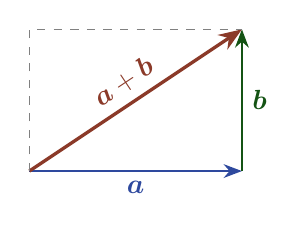
\begin{tikzpicture}[>=Stealth, scale=0.9]
  \draw[->,thick,RoyalBlue!70!black] (0,0) -- (3,0)
        node[midway,below] {$\vect{a}$};
  \draw[->,thick,ForestGreen!60!black] (3,0) -- (3,2)
        node[midway,right] {$\vect{b}$};
  \draw[->,very thick,BrickRed!70!black] (0,0) -- (3,2)
        node[midway,above,sloped] {$\vect{a}+\vect{b}$};
  \draw[dashed,gray] (0,0) -- (0,2) -- (3,2);
\end{tikzpicture}
\end{center}

The dashed lines show the equivalent \textbf{parallelogram rule}:
$\vect{a}+\vect{b}$ is the diagonal of the parallelogram built from $\vect{a}$ and $\vect{b}$.

\subsection*{Mathematical expression}

\begin{mathblock}{Rule}
Vectors add componentwise:
\[
  \vect{a} + \vect{b}
  \;=\;
  (a_1, a_2, \dots, a_n) + (b_1, b_2, \dots, b_n)
  \;=\;
  (a_1+b_1,\; a_2+b_2,\; \dots,\; a_n+b_n).
\]
\end{mathblock}

So $(3,0) + (0,4) = (3,4)$, with magnitude $5$. You walked $3+4 = 7$ steps in total,
but your \emph{displacement} from the start is only $5$ steps. That gap is exactly
why scalars cannot describe walking direction.

Vector addition is \textbf{commutative} ($\vect{a}+\vect{b} = \vect{b}+\vect{a}$)
and \textbf{associative}, just like number addition. There is a \textbf{zero vector}
$\vect{0} = (0,\dots,0)$ with no length and no direction; adding it changes nothing.

\section{Q4: multiplying a vector by a number}

\subsection*{Naive intuition}

If $\vect{v}$ is an arrow, then $2\vect{v}$ is the arrow pointing the \emph{same way}
but \emph{twice as long}. The arrow $-\vect{v}$ is the same length as $\vect{v}$
but points in the \emph{opposite} direction. The number doing the stretching or flipping
is called a \textbf{scalar} --- this is where the word comes from.

\subsection*{Mathematical expression}

\begin{mathblock}{Rule}
For a scalar $\lambda \in \mathbb{R}$ and a vector $\vect{v} = (v_1,\dots,v_n)$,
\[
  \lambda \vect{v} \;=\; (\lambda v_1,\; \lambda v_2,\; \dots,\; \lambda v_n),
  \qquad
  \lVert \lambda \vect{v} \rVert \;=\; \lvert \lambda \rvert \cdot \lVert \vect{v} \rVert.
\]
\end{mathblock}

Combined with addition, this gives the very useful operation of writing one vector
as a \textbf{linear combination} of others: any 2D vector can be written as
$\vect{v} = v_1 \vhat{i} + v_2 \vhat{j}$.

\section{Two ways to multiply two vectors}

Adding two vectors gives another vector. Multiplying two vectors is more interesting:
there are two genuinely useful definitions, and physics uses both.

\subsection{The dot product (a number)}

\begin{mathblock}{Definition}
\begin{definition}
The \textbf{dot product} of $\vect{a}$ and $\vect{b}$ is the scalar
\[
  \vect{a}\cdot\vect{b}
  \;=\; a_1 b_1 + a_2 b_2 + \dots + a_n b_n
  \;=\; \lVert\vect{a}\rVert\,\lVert\vect{b}\rVert \cos\theta,
\]
where $\theta$ is the angle between the two arrows.
\end{definition}
\end{mathblock}

In words: the dot product measures \emph{how much of $\vect{a}$ points in the
direction of $\vect{b}$}, scaled by their lengths. If the two vectors are
perpendicular, $\cos\theta = 0$ and the dot product is zero. This is exactly the
test physicists use for ``these two directions are independent''.

\subsection{The cross product (another vector, in 3D)}

\begin{mathblock}{Definition}
\begin{definition}
For $\vect{a},\vect{b}\in\mathbb{R}^3$, the \textbf{cross product} $\vect{a}\times\vect{b}$
is the vector
\begin{itemize}
  \item with magnitude $\lVert\vect{a}\rVert\,\lVert\vect{b}\rVert \sin\theta$
        (the area of the parallelogram spanned by $\vect{a}$ and $\vect{b}$);
  \item perpendicular to \emph{both} $\vect{a}$ and $\vect{b}$;
  \item pointing in the direction given by the right-hand rule.
\end{itemize}
In components,
\[
  \vect{a}\times\vect{b}
  \;=\;
  (a_2 b_3 - a_3 b_2,\; a_3 b_1 - a_1 b_3,\; a_1 b_2 - a_2 b_1).
\]
\end{definition}
\end{mathblock}

The cross product is special to three dimensions and is the natural language
for \emph{rotation}: torque, angular momentum and magnetic forces are all defined this way.

\section{A basic theorem worth remembering}

\begin{mathblock}{Theorem (triangle inequality)}
\begin{theorem}
For any two vectors $\vect{a}$ and $\vect{b}$,
\[
  \lVert \vect{a} + \vect{b} \rVert \;\le\; \lVert \vect{a} \rVert + \lVert \vect{b} \rVert,
\]
with equality if and only if $\vect{a}$ and $\vect{b}$ point in the same direction.
\end{theorem}
\end{mathblock}

\begin{mathblock}{Why it is true (sketch)}
\begin{proof}
Square the left-hand side and use the dot product:
\[
  \lVert\vect{a}+\vect{b}\rVert^2
  = (\vect{a}+\vect{b})\cdot(\vect{a}+\vect{b})
  = \lVert\vect{a}\rVert^2 + 2\,\vect{a}\cdot\vect{b} + \lVert\vect{b}\rVert^2.
\]
Since $\vect{a}\cdot\vect{b} = \lVert\vect{a}\rVert\,\lVert\vect{b}\rVert\cos\theta
\le \lVert\vect{a}\rVert\,\lVert\vect{b}\rVert$, the right-hand side is at most
$(\lVert\vect{a}\rVert+\lVert\vect{b}\rVert)^2$. Take the square root.
Equality needs $\cos\theta = 1$, i.e.\ same direction.
\end{proof}
\end{mathblock}

The intuition: the straight path from start to end is never longer than going via a detour.
Walking east and then north covers more distance than going diagonally to the same endpoint.

\section{A worked example}

\begin{mathblock}{Example}
\begin{example}
Two forces act on a small box on a frictionless floor:
$\vect{F}_1 = (4, 0)$~N (a $4$~N push to the east)
and $\vect{F}_2 = (0, 3)$~N (a $3$~N push to the north).
Find the total force and its direction.
\end{example}
\end{mathblock}

\textbf{Solution.}
The total force is the vector sum
\[
  \vect{F} \;=\; \vect{F}_1 + \vect{F}_2 \;=\; (4,0) + (0,3) \;=\; (4,3)~\text{N}.
\]
Its magnitude is
\[
  \lVert \vect{F} \rVert = \sqrt{4^2 + 3^2} = 5~\text{N}.
\]
Its direction makes an angle $\theta$ above the east axis, where
\[
  \tan\theta = \frac{3}{4}, \qquad \theta \approx 36.87^\circ.
\]
So the box accelerates along a $5$~N force aimed about $37^\circ$ north of east.
A scalar alone could never have told us the direction; that is why physics uses vectors.

\section{Where vectors actually live in physics}

\begin{problemblock}
What kinds of physical quantities are vectors, and where do they appear?
\end{problemblock}

\subsection*{Kinematics: position, velocity, acceleration}

\begin{solutionblock}
The \textbf{position} of a particle relative to an origin is a vector
$\vect{r}(t) = (x(t), y(t), z(t))$.
Its time derivative is the \textbf{velocity}
$\vect{v}(t) = \tfrac{d\vect{r}}{dt}$,
and the derivative of velocity is the \textbf{acceleration}
$\vect{a}(t) = \tfrac{d\vect{v}}{dt}$.
All three carry direction information that scalars cannot.
\end{solutionblock}

\subsection*{Dynamics: Newton's second law}

\begin{solutionblock}
Newton's second law is a \emph{vector} equation:
\[
  \vect{F}_{\text{net}} \;=\; m\,\vect{a}.
\]
The net force and the resulting acceleration always point in the same direction
(because $m > 0$ is a scalar). When several forces act, the rule is
$\vect{F}_{\text{net}} = \sum_i \vect{F}_i$ --- exactly the vector addition we drew above.
\end{solutionblock}

\subsection*{Momentum and angular momentum}

\begin{solutionblock}
Linear momentum is $\vect{p} = m\vect{v}$, a vector.
Angular momentum about an origin is the cross product
\[
  \vect{L} \;=\; \vect{r} \times \vect{p},
\]
and torque is $\vect{\tau} = \vect{r}\times\vect{F}$.
The cross product is what encodes ``rotation about an axis''; the direction of
$\vect{L}$ is the rotation axis itself, by the right-hand rule.
\end{solutionblock}

\subsection*{Work and energy}

\begin{solutionblock}
The \textbf{work} done by a constant force $\vect{F}$ along a displacement $\vect{d}$ is
\[
  W \;=\; \vect{F}\cdot\vect{d} \;=\; \lVert\vect{F}\rVert\,\lVert\vect{d}\rVert\cos\theta.
\]
Only the component of the force \emph{along} the motion does work --- and that is
exactly what the dot product measures. A force perpendicular to the motion
(such as the centripetal force on a planet in a circular orbit) does no work.
\end{solutionblock}

\subsection*{Fields: gravity, electricity, magnetism}

\begin{solutionblock}
A \textbf{vector field} assigns a vector to every point in space.
The gravitational field $\vect{g}(\vect{r})$ tells you the direction and strength of
gravity at each point. The electric field $\vect{E}(\vect{r})$ pushes a charge $q$
with force
\[
  \vect{F} \;=\; q\,\vect{E}.
\]
A moving charge in a magnetic field $\vect{B}$ feels the \textbf{Lorentz force}
\[
  \vect{F} \;=\; q\,\vect{v}\times\vect{B},
\]
which uses the cross product and explains why charged particles spiral around field lines.
\end{solutionblock}

\subsection*{Beyond elementary mechanics}

\begin{solutionblock}
Once you know vectors, the same idea generalises:
\begin{itemize}
  \item \textbf{Tensors} in general relativity are higher-rank cousins of vectors.
  \item In quantum mechanics, the \emph{state} of a system is a vector in a
        complex inner-product space (a Hilbert space), and the dot product
        becomes the inner product $\langle \psi | \phi \rangle$.
  \item Conservation laws (momentum, angular momentum) are most naturally
        stated as ``a certain vector does not change with time''.
\end{itemize}
\end{solutionblock}

\section{What to remember}

\begin{enumerate}[label=\textbf{\arabic*.}]
  \item A vector is a \emph{quantity with both magnitude and direction};
        a scalar is just a number.
  \item In coordinates, a vector is an ordered tuple $(v_1,\dots,v_n)$;
        each entry is ``how much of that axis''.
  \item Vectors add tip-to-tail (componentwise); scalars stretch them.
  \item The dot product extracts ``how much one vector points along another''
        and is the language of \emph{work} and \emph{projection}.
  \item The cross product (in 3D) builds a perpendicular vector and is the
        language of \emph{rotation}: torque, angular momentum, magnetism.
  \item Physics is full of vector quantities: position, velocity, acceleration,
        force, momentum, angular momentum, electric and magnetic fields.
        Newton's second law $\vect{F} = m\vect{a}$ is itself a vector equation.
\end{enumerate}

\begin{keypointblock}
A vector is the smallest object that can answer ``how much, and in which direction?''
--- and once you have it, almost every law in classical physics turns out to be a
sentence about vectors.
\end{keypointblock}

\end{document}
